\documentclass[11pt]{amsart}
\usepackage[margin=1.1in]{geometry}
\usepackage{amsmath,amssymb,amsthm,booktabs,graphicx}
\usepackage[colorlinks=true,allcolors=blue]{hyperref}
\newtheorem{theorem}{Theorem}
\newtheorem{proposition}[theorem]{Proposition}
\newtheorem{lemma}[theorem]{Lemma}
\theoremstyle{remark}
\newtheorem{remark}[theorem]{Remark}
\begin{document}
\title[Fully clued Slitherlink with five solutions]{A fully clued Slitherlink diagram with exactly five solutions}
\author{Zijian Zeng}
\address{UCSI University, Kuala Lumpur, Malaysia}
\date{18 November 2026}
\begin{abstract}
When every cell of a Slitherlink diagram carries a clue, the clues are the \emph{signature} of a loop, and the
puzzle can still have several solutions. Knuth's answer to exercise 7.2.2.1--411 of \emph{The Art of Computer
Programming}, as amended in August 2023, reports N.~Beluhov's fully clued diagrams with exactly three solutions and
states that it is unknown whether exactly five solutions are possible; Beluhov asked more generally whether five or
more are possible. We give a fully clued $13\times13$ diagram with exactly five solutions, and fully clued $12\times12$
and $13\times13$ diagrams with exactly six. Exhaustive searches show that every fully clued diagram with fewer than
$144$ cells has at most four solutions, so the $12\times12$ example has the least possible area. Each count was
confirmed by independent programs.
\end{abstract}
\maketitle

\section{The question and the answer}
An $m\times n$ Slitherlink diagram has $m\times n$ square cells, and a solution is a single closed loop along the
grid lines that passes exactly $k$ sides of every cell clued $k$. If every cell is clued, the clues are determined by
the loop; following Beluhov~\cite{beluhov} we call them the \emph{signature} of the loop, and the number of loops with
a given signature its \emph{multiplicity}. Exercise 7.2.2.1--411 of~\cite{knuth4b} asks whether a fully clued diagram
can have more than one solution; it can, and Knuth's answer gives a $6\times6$ example with four. Beluhov~\cite{beluhov}
proved that every $m\times n$ diagram is unambiguous when $\gcd(m+1,n+1)=1$ and constructed infinitely many fully
clued square diagrams with exactly three and with exactly four solutions. (Beluhov measures grids by vertices; his
$7\times7$ and $8\times8$ grids are the $6\times6$ and $7\times7$ diagrams here.) Knuth's amendment of 28 August 2023
to answer 411~\cite{errata4b} ends with the sentence ``It's currently unknown whether or not exactly five loops are
possible,'' and Section~10 of~\cite{beluhov} lists the existence of a signature of multiplicity at least five as an
open problem.

\begin{theorem}\label{thm:five}
The fully clued $13\times13$ diagram of Fig.~\ref{fig:five} has exactly five solutions.
\end{theorem}

\begin{theorem}\label{thm:six}
The fully clued $12\times12$ diagram of Fig.~\ref{fig:six} and the $13\times13$ diagram~\eqref{eq:six13} have
exactly six solutions each.
\end{theorem}

\begin{proposition}\label{prop:small}
Every fully clued diagram with fewer than $144$ cells has at most four solutions. In particular no fully clued
$n\times n$ diagram with $n\le11$ has five or more.
\end{proposition}

Thus every multiplicity from $1$ to $6$ occurs, and the $12\times12$ diagram of Fig.~\ref{fig:six} has the least
area among diagrams with five or more solutions. Whether some $12\times12$ diagram has exactly five solutions is not
yet settled, so the least area for exactly five is $144$ or $169$.

\begin{figure}[ht]
\centering
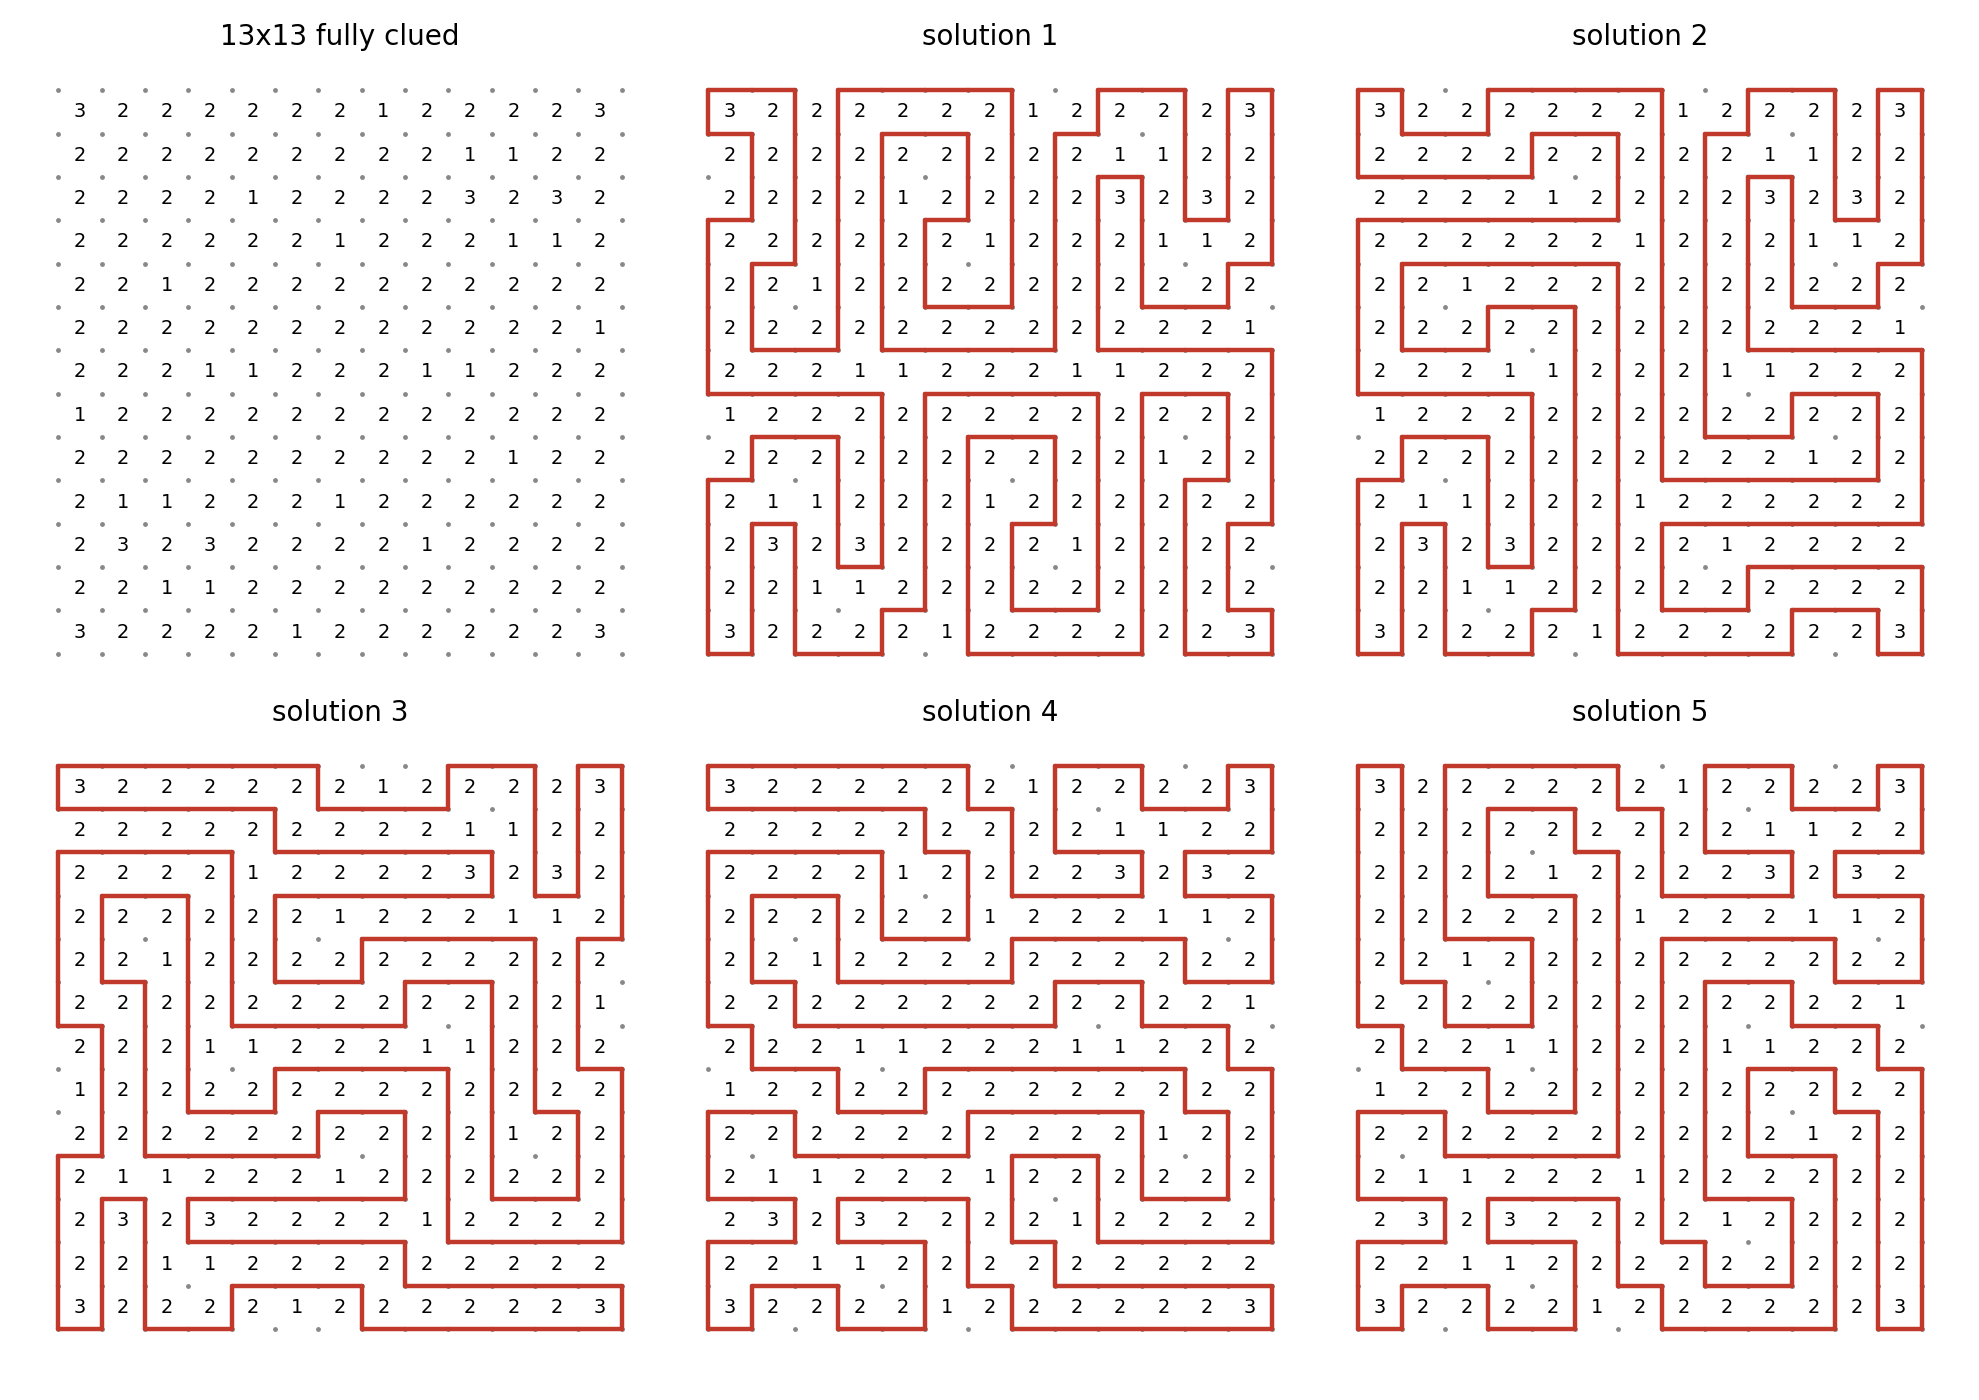
\includegraphics[width=0.94\textwidth]{m5_13x13.png}
\caption{A fully clued $13\times13$ diagram (top left) and its five solutions.}\label{fig:five}
\end{figure}

The clues of Fig.~\ref{fig:five}, row by row from the top, are
\begin{equation}\label{eq:five}
\begin{array}{l}
\texttt{3222222122223}\ \texttt{2222222221122}\ \texttt{2222122223232}\ \texttt{2222221222112}\ \texttt{2212222222222}\\
\texttt{2222222222221}\ \texttt{2221122211222}\ \texttt{1222222222222}\ \texttt{2222222222122}\ \texttt{2112221222222}\\
\texttt{2323222212222}\ \texttt{2211222222222}\ \texttt{3222212222223}.
\end{array}
\end{equation}

\begin{figure}[ht]
\centering
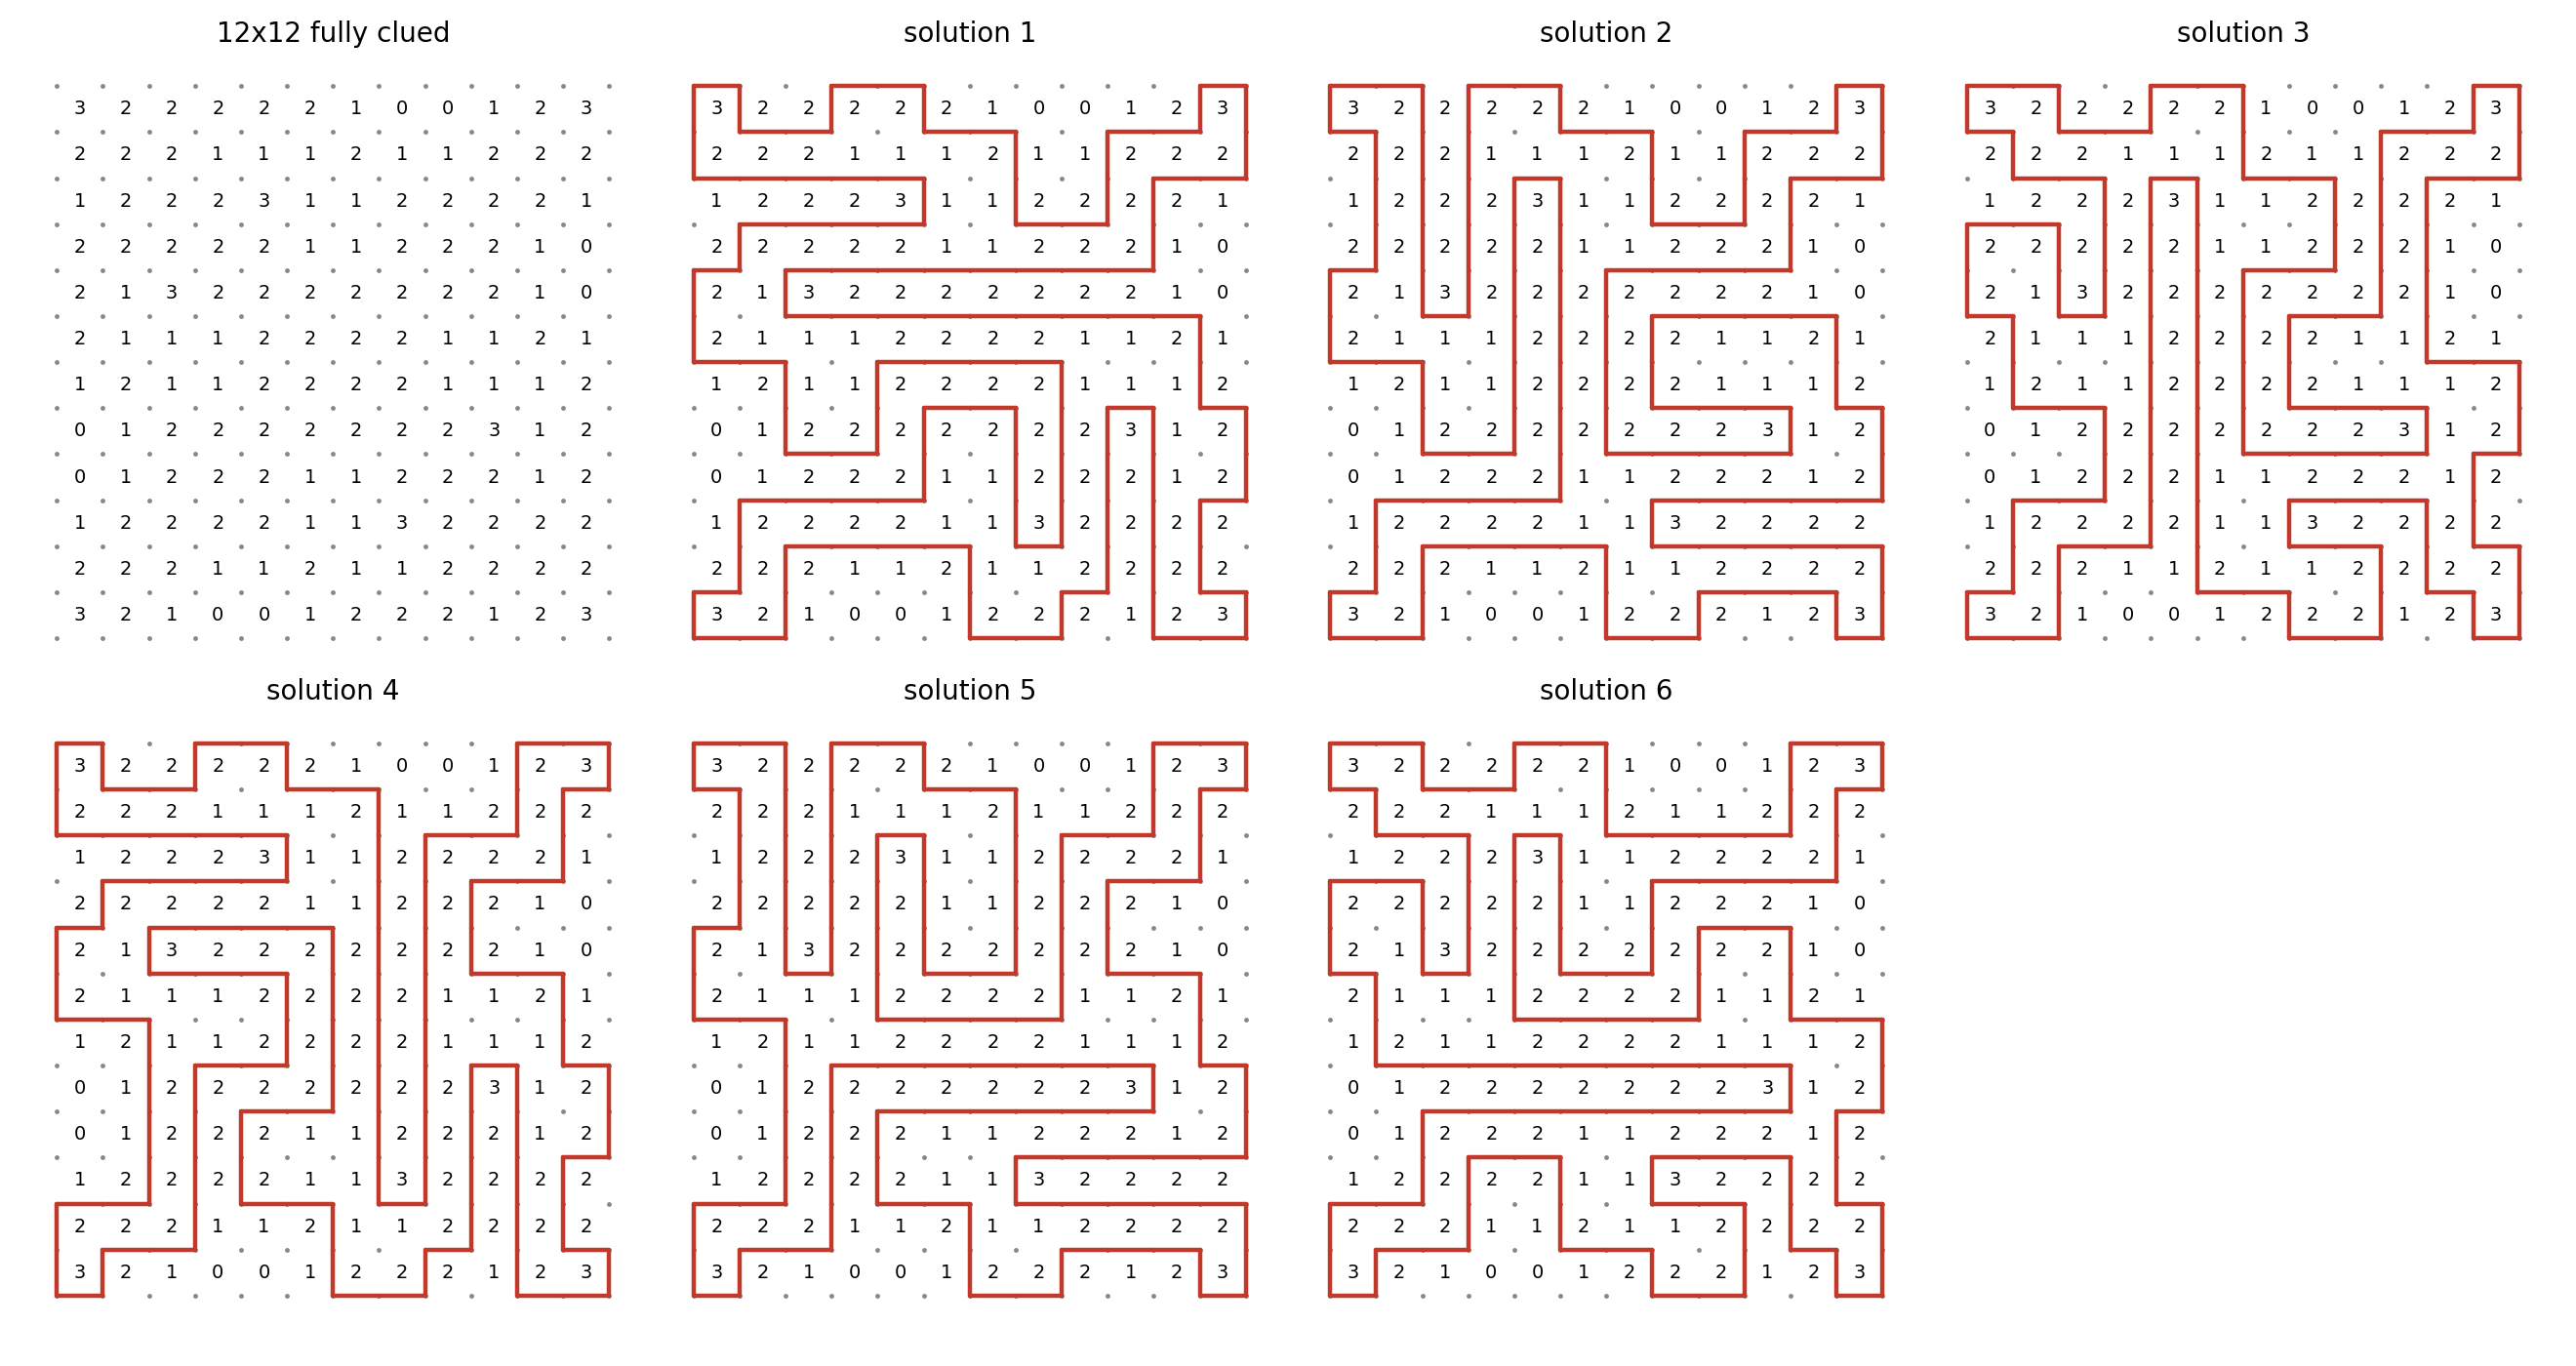
\includegraphics[width=0.94\textwidth]{m6_12x12.png}
\caption{A fully clued $12\times12$ diagram (top left) and its six solutions.}\label{fig:six}
\end{figure}

The clues of Fig.~\ref{fig:six} are
\texttt{322222100123}, \texttt{222111211222}, \texttt{122231122221}, \texttt{222221122210},
\texttt{213222222210}, \texttt{211122221121}, \texttt{121122221112}, \texttt{012222222312},
\texttt{012221122212}, \texttt{122221132222}, \texttt{222112112222}, \texttt{321001222123}; and a $13\times13$ diagram
with six solutions is
\begin{equation}\label{eq:six13}
\begin{array}{l}
\texttt{3222221132222}\ \texttt{2221112122312}\ \texttt{1222311221112}\ \texttt{2222211221121}\ \texttt{2132222112210}\\
\texttt{2111222112210}\ \texttt{1211222221121}\ \texttt{0122112221112}\ \texttt{0122112222312}\ \texttt{1211221122222}\\
\texttt{2101221132221}\ \texttt{2012112111222}\ \texttt{2221001222223}.
\end{array}
\end{equation}

\section{Totally even sets}
Let $G$ be the grid of an $m\times n$ diagram, with $(m+1)(n+1)$ vertices. Following~\cite[\S4]{beluhov}, a set $E$
of edges of $G$ is \emph{totally even} if every vertex and every cell meets an even number of edges of~$E$. If two
loops $L_1$, $L_2$ have the same signature, then $L_1\oplus L_2$ (symmetric difference) is totally even, since at
every vertex both loops have degree $0$ or $2$ and every cell contains equally many edges of $L_1$ and of $L_2$.

The totally even sets form a vector space $T$ over $\mathbb F_2$, and $\dim T=\gcd(m+1,n+1)-1$
\cite[\S4]{beluhov}. Here is a short way to see this. A totally even set $E$ has even degree at every vertex, so it
is the boundary $\partial S$ of a unique set $S$ of cells. A cell $x$ contains $|N(x)\cap S|$ edges of $\partial S$ if
$x\notin S$ and $4-|N(x)\cap S|$ if $x\in S$, where $N(x)$ is the set of cells adjacent to $x$; so $E$ is totally even
if and only if $S$ lies in the kernel of the adjacency matrix of the $m\times n$ grid graph over $\mathbb F_2$, whose
nullity is $\gcd(m+1,n+1)-1$ over every field \cite{tomei}, \cite[\S4]{beluhov}. In particular a signature has multiplicity at most $2^{\dim T}$, so five
or more solutions require $\gcd(m+1,n+1)\ge4$.

By \cite[Lemma~2]{beluhov} a totally even set is determined by the edges it contains along one side of the grid. For
$n\times n$ diagrams we write $B(i)$, $1\le i\le n$, for the totally even set that contains exactly the $i$th edge from
the left of the bottom side; these are Beluhov's diamond sets, and they form a basis of $T$.

A loop $L$ and a set $E\in T$ give a solution $L\oplus E$ of the signature of $L$ exactly when (a) every cell
contains equally many edges of $E\cap L$ and of $E\setminus L$, and (b) $L\oplus E$ is a single loop. So the solutions
of the signature of $L$ are the loops $L\oplus E$ for $E$ in
$D(L)=\{E\in T: \text{(a) and (b) hold}\}$, and the multiplicity is $|D(L)|$.

\section{The search}
Call $E\in T\setminus\{0\}$ \emph{feasible} if some nonempty edge set $P$ with all degrees $0$ or $2$ has
$P\oplus E$ of the same kind and condition~(a) holds. If a signature has solutions $L=L_0,L_1,\dots,L_{k-1}$, then
the sets $E_i=L\oplus L_i$ are distinct, nonzero and feasible (with witness $L$), and so is every
$E_i\oplus E_j=L_i\oplus L_j$ (with witness $L_i$). So $\{E_1,\dots,E_{k-1}\}$ is a clique in the graph on the feasible
sets in which $E$ and $F$ are adjacent when $E\oplus F$ is feasible. The search therefore
\begin{enumerate}
\item computes a basis of $T$ by Gaussian elimination over $\mathbb F_2$ and tests each nonzero set for feasibility
with a SAT solver;
\item enumerates all $(k-1)$-cliques of the feasibility graph;
\item for each clique, solves one SAT model whose variables describe $L$: degree $0$ or $2$ at every vertex for $L$ and
for every $L\oplus E_i$, condition~(a) for every $E_i$, and single-loop conditions added lazily (when a model has a copy
with two components $C,C'$, no copy may contain all of $C\cup C'$; a single loop never contains two disjoint loops);
\item computes the exact multiplicity of every signature found.
\end{enumerate}
A cap on the number of lazy iterations is logged when reached; it was never reached in the searches used below.

For $k=5$ and $n\times n$ diagrams with $3\le n\le11$ there are respectively $2,7,8,20,25,54,72,143,205$ feasible sets
(out of $2^n-1$) and $0,0,0,140,245,6825,14875,194775,520320$ cliques of size four, and no clique model has a solution
in which all five copies are single loops. The same holds for all $35$ non-square $m\times n$ diagrams with
$3\le m<n$, $mn\le171$ and $\gcd(m+1,n+1)\ge4$. Diagrams with $\gcd(m+1,n+1)\le3$ have multiplicity at most~$4$, so
Proposition~\ref{prop:small} follows. With $k=4$ and $k=3$ the same program immediately finds Knuth's $6\times6$
diagram with four solutions and a $7\times7$ diagram with three, the smallest square cases reported
in~\cite{beluhov}. On the $13\times13$ grid a partial run with $k=5$ (not yet finished) has found $68$ inequivalent signatures
of multiplicity five and $220$ of multiplicity six; they are listed with the programs.

\section{Verification and structure}
The multiplicities in Theorems~\ref{thm:five} and~\ref{thm:six} were computed in four ways, by two independent
groups of programs:
\begin{itemize}
\item a SAT enumeration of all single-loop solutions, with lazy cuts against unions of loops;
\item a plain backtracking program in C that assigns the edges one at a time, prunes only by clues and vertex
degrees, and checks connectivity with union--find (it uses neither SAT nor totally even sets);
\item an exact frontier dynamic program over the vertices, validated against complete cycle enumeration on small
grids; and
\item enumeration of $L\oplus E$ over all $E\in T$ from every solution $L$.
\end{itemize}
The last two, and an independent exhaustive search confirming Proposition~\ref{prop:small} (backtracking over all
loops while keeping the set of $E\in T$ that remain consistent), were written by a separate referee without access to
the first two. All four give exactly $5$ for~\eqref{eq:five}, exactly $6$ for the other two diagrams, and $4$ for
Knuth's $6\times6$ example.

Relative to the first loop of Fig.~\ref{fig:five}, the five solutions differ by
$0$, $X$, $Y$, $Y\oplus Z$, $Y\oplus Z\oplus X$, where $X=B(12)$, $Y=B(7)\oplus B(11)$ and $Z=B(3)\oplus B(5)$.
That is, $D(L)=\{0,Y,Y\oplus Z\}\cup\bigl(X\oplus\{0,Y\oplus Z\}\bigr)$: a three-way choice, together with a switch
$X$ that is available in only two of the three states, giving $3+2=5$. Relative to the first loop of
Fig.~\ref{fig:six}, $D(L)=\{0,B(2)\}\oplus\{0,B(11),B(7)\oplus B(9)\oplus B(11)\}$, a two-way switch combined with a
three-way choice of the kind that gives Beluhov's diagrams of multiplicity three; diagram~\eqref{eq:six13} has the
same form, $\{0,B(1)\oplus B(3)\}\oplus\{0,B(8)\oplus B(10),B(8)\oplus B(10)\oplus B(12)\}$.

\begin{remark}
It remains open which positive integers occur as multiplicities; the partial runs on $13\times13$, $14\times14$ and
$15\times15$ grids have found no multiplicity above six. The least area of a diagram with exactly five solutions is
$144$ or $169$.
\end{remark}

\subsection*{How this was done}
The searches, the first two counters and this note were produced by Claude (Anthropic's AI model) at the author's
direction; the other two counters and the confirming search were written by a separate AI agent acting as referee,
which had no access to the first programs until its counts were done. No human expert has checked the results yet.
All programs, logs, the diagrams and their loops (in machine-readable form) are public at
\url{https://github.com/ArtificialZeng/AI-Has-Taste}.

\begin{thebibliography}{9}
\bibitem{beluhov} N. Beluhov, \emph{Slitherlink signatures}, arXiv:2308.08798 [math.CO] (2023), 28 pages.
\bibitem{knuth4b} D. E. Knuth, \emph{The Art of Computer Programming}, Vol.~4B: Combinatorial Algorithms, Part~2
(Addison--Wesley, 2022), \S7.2.2.1, exercise 411 and its answer.
\bibitem{errata4b} D. E. Knuth, Errata for Volume 4B (1st ed.), \url{https://cs.stanford.edu/~knuth/all4b.ps.gz},
amendment to page 535 dated 28 August 2023 (file last updated 16 April 2026).
\bibitem{tomei} C. Tomei and T. Vieira, The kernel of the adjacency matrix of a rectangular mesh, \emph{Discrete
Comput. Geom.} \textbf{28} (2002), no.~3; arXiv:math/0201211.
\end{thebibliography}
\end{document}
